\chapter{Algebra Part I}

\subsection{Worksheet 1E: Warm-Up Problems}

\textbf{Write the strategy that is best used to solve the problem and then solve it.}

\begin{multienumerate}
\mitemxx{\basic

A car rental company has two policies. Policy A requires customers to pay a monthly \$75 fee and an additional \$6 for every hour they use the car. Policy B has no monthly fee but requires customers to pay \$11 for every hour they use the car. How many hours does a customer have to drive in a month to make policy A more advantageous than policy B?

\bigskip
Strategy:

\bigskip
Solve:
}{\medium

John places an order at a local pizzeria for $p$ total pizzas. Where $p$ is at least 4 but no more than 6, which inequality represents all possible values of $p$?

\begin{enumerate}[label=(\Alph*)]
\item $|p-5|\leq2$
\item $|p-5|\leq1$
\item $|p-1|\leq6$
\item $|2-p|\leq4$
\item $|2-p|\leq1$
\end{enumerate}

\bigskip
Strategy:

\bigskip
Solve:}

\vfill
\mitemx{\medium

Ella has a group of friends consisting of both 1st and 3rd graders. One day she decides to invite all 8 of them over for a tea party. At the party she plans to bake cookies for all of her friends. Naturally, the 3rd graders can eat 5 cookies each and the 1st graders only eat 2 cookies each. Using this information, Ella estimates how many cookies her friends will eat and then makes 10 extra just in case people eat more. If she made 32 cookies, how many 1st grade friends are coming?

\begin{enumerate}[label=(\Alph*)]
\item 8
\item 7
\item 6
\item 5
\item 4
\end{enumerate}

\bigskip
Strategy:

\bigskip
Solve:}
\end{multienumerate}

\newpage
\section[Functions]{Algebra Topic \#1: Functions}

Connection to previous material learned:

\begin{itemize}
\item If $y=x^2-1$ and $x=-2$ what is the value of $y$? \longline
\item If $y=1-x$ and $y=-2$, what is the value of $x$? \longline
\item A problem-solving strategy to keep in mind: If you have a problem with lots of variables and don't know how to solve it, you should try to \longline the answer choices to help you solve the problem. For example, we could \longline for each variable, plug in this number into the problem and each of the answer choices, and solve to see which solution of the answer choices \longline the solution in the question.
\end{itemize}

\vfill
Functions have the form $f(x)=$ some definition with an $x$, such as $f(x)=x^2-1$. The notation for a function is a letter and $x$ combination, $f(x)$ and $g(x)$. Both can be treated as $y$, so ``If $y=x^2-1$ and $x=-2$, what is the value of $y$?” becomes ``If $f(x)=x^2-1$ and $x=-2$, what is the value of $f(x)$?'' and ``if $g(x)=1-x$ and $g(x)=-2$, what is the value of $x$?'' \longline

\vfill
The variable in the parentheses is what gets plugged in to the definition. For example, $f(2)=x^2-1$ can be written as $f(2)=$\longline. Now solve $f(2)=x^2-1$ to get an answer of \longline. You may also get questions that give you the value of the output, f(2), and ask you to find the variable, $x$. Therefore, if the value of $f(x)=3$ and the definition of $f(x)=x^2-1$, what is $x$? \longline.

\vfill
Sometimes you may be given the input and output ($x$ and $f(x)$) and then be expected to find the equation or part of an equation, such as a coefficient or a constant in the equation. To do so, plug in the numbers given in the problem and solve for the unknown.

\vfill
What should you do when you have two functions in the same problem? The output of one function can solve as the input for another function. For example, if $f(x)=x+1$ and $g(x)=2x$, then what is $g(f(x))$? To find this, start with the \longline. In this example, we can find the value of $f(x)$. Then plug this output into the x value of the function on the outside. Using $f(x)$ and $g(x)$ defined earlier in this paragraph, what is $f(g(2))$? What is $g(f(2))$? \longline

\vfill
The SATs will also define novel functions with a weird symbol $-$ such as $\diamond$, $\uparrow$, \$, etc. $-$ and ask you to then solve for some part of the function. These are often called ``weird symbol problems''. Most of the time, you need to solve the equation that they give you using the number in the problem. For example, if $\#g\#=g+1$, then what is \#5\#? \longline If $\#g\#h\#=gh-h$, then what is \#5\#6\#? \longline.

\newpage
\subsection{SAT Worksheet 2E: 8 Questions, 10 Minutes}

\begin{multienumerate}
\mitemxx{\basic

If $f(x)=(3-4x^2)/-1$, what is the value of $f(-1)$?

\begin{enumerate}[label=(\Alph*)]
\item $-1$
\item 0
\item 1
\item 2
\item 4
\end{enumerate}
}{\basic

If $f(x)=x^2-1$, what is the value of $2f(5)$?
\begin{enumerate}[label=(\Alph*)]
\item 4
\item 10
\item 24
\item 48
\item 25
\end{enumerate}}

\vfill
\mitemxx{\medium

If $f(p)=(2p)^2-5$ and $f(p)=10$, what is the value of $f(p^2)$?}{\medium

Let $f$ be a function such that $f(x)=c|x^3|+12$ where $c$ is a constant. If $f(-1)=4$, what is the value of $f(5)$?}

\vfill
\mitemxx{\advanced

If $f(x)=-2x+8$, give a value of $x$ for which $f(x)=2f(x)$.}{\advanced

In the function $g(x)=ax^2+5$, $a$ is a constant. When graphed on the $xy$-coordinate plane, one of the points on the line is $(4,6)$. What is the value of the constant $a$?}

\vfill
\mitemxx{\advanced

If $f(x)=x^2-2x+9$ and $g(x)=|x|+$, what is $f(g(-10))$?}{\advanced

If $f(x)=x+4$ and $g(x)=5(x)-2(x)$, what is the positive difference between $f(g(2))$ and $g(f(2))$?}
\end{multienumerate}

\vfill
\newpage
\section{Functions with Charts and Graphs}

Sometimes, there are questions with charts containing the input, x, and the corresponding output, f(x). These questions will usually ask you to find the equation that fits the line of the \longline.

\bigskip
In order to solve these types of problems, you will need to plug x and f(x) into the equation given or in the answer choices. Most of the time, you will need to check that the equation with \longline points rather than just one because more than one answer choice will work for one pair of $x$ and $f(x)$ values.

\bigskip
Example \#1: given the chart of the quadratic function below, what is the general equation of the function?

\bigskip
\begin{spacing}{1.5}
\begin{tabularx}{\textwidth}{|*6{@{}>{\centering\arraybackslash$}X<{$\arraybackslash}|}}\hline
x & -2 & -1 & 0 & 1 & 2\\\hline
f(x) & 5 & 2 & 1 & 2 & 5\\\hline
\end{tabularx}
\end{spacing}

\section{Functions and Graphs}

Functions may be graphed on an $xy$-coordinate plan. Remember that in the form of the function $f(x)$, the value of $x$ in the $f(x)$ is plotted on the $x$-coordinate and the value of $f(x)$ is treated as the $y$-coordinate.

\begin{enumerate}
\item Graph the quadratic function given in example \#1 above:

\plane

\item What is the minimum of the function?
\item Use the graph to find $f(2)$.
\item Use the graph to find $x$ when $f(x)=2$
\end{enumerate}

The SATs will often ask about transformations of the graph of a function. Determine how each of the following transformations will affect a function. Then, draw the transformation of the function $f(x)=x^2+1$ on the grid beside the transformation.

\begin{multicols}{2}
\textbf{Reflection in the $\boldsymbol{x}$-axis}

\bigskip
For example: $f(x)\rightarrow-f(x)$

\vfill
\columnbreak
\plane
\end{multicols}

\hrulefill
\begin{multicols}{2}
\textbf{Vertical Translation}

Move $f(x)$ up or down on the $y$-axis

\bigskip
For example: $f(x)\rightarrow f(x)+2$

\vfill
\columnbreak
\plane
\end{multicols}

\hrulefill
\begin{multicols}{2}
\textbf{Horizontal Translation}

Move $f(x)$ to the left or the right (move the function along the $x$-axis)

\bigskip
For example: $f(x-2)$

\vfill
\columnbreak
\plane
\end{multicols}

\newpage
\begin{multicols}{2}
\textbf{Vertical Stretch/Compression}

\bigskip
For example: $f(x)\rightarrow2f(x)$

\vfill
\columnbreak
\plane
\end{multicols}

\hrulefill
\begin{multicols}{2}
\textbf{Horizontal Stretch/Compression}

\bigskip
For example: $f(x)\rightarrow f(2x)$

\vfill
\columnbreak
\plane
\end{multicols}

\newpage
\subsection{SAT Worksheet 3E: 6 Questions, 8 Minutes}

\begin{multienumerate}
\mitemxx{\basic

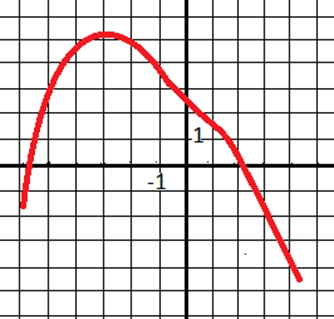
\includegraphics{50}

Based on the graph of the function $g$ above, for what values of $x$ is $g(x)$ positive?}{\basic

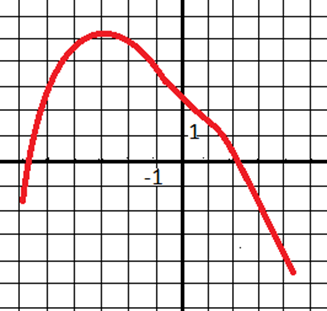
\includegraphics{51}

The graph above contains the function $f(b)$. If $f(b)=0$, which of the following is a possible value for $b$?

\begin{enumerate}[label=(\Alph*)]
\item $-1$
\item 0
\item 1
\item 2
\item 5
\end{enumerate}}

\vfill
\mitemxx{\medium

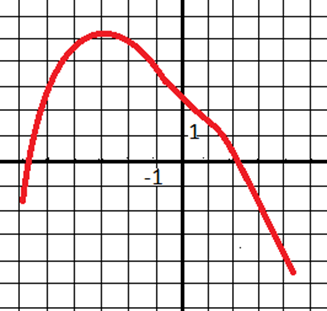
\includegraphics{51}

The graph above contains the functions $f(x)$ and $g(x)$. If $g(5)=b$, what is the value of $f(b)$?
}{\medium

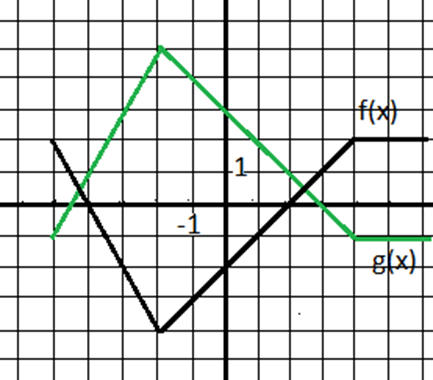
\includegraphics{52}

The graph above contains the functions $f(x)$ and $g(x)$. Which of the following equations best represents the relationship between $f(x)$ and $g(x)$?

\begin{enumerate}[label=(\Alph*)]
\item $f(x)=-g(x)+1$
\item $f(x)=-g(x-1)$
\item $f(x)=-g(x)$
\item $f(x)=2g(x)$
\item $f(x)=-g(x)-1$
\end{enumerate}}

\vfill
\mitemxx{\advanced

If $f(x)=x^2-2x$, then how will a graph of $f(x+2)$ differ from a graph of $f(x)$?

\begin{enumerate}[label=(\Alph*)]
\item Stretched by a factor of 2
\item Shifted right by 2
\item Increased by 2
\item Compressed by a factor of 2
\item No change
\end{enumerate}
}{\advanced

Let the function $g$ be defined by $g(a)=-3a$. If $3/5g(a^{1/2})=12$, what is the value of $a$?}
\end{multienumerate}

\section[Word Problems]{Functions and Equations in Word Problems}

Given the equation and asked to solve for the input or output or you may be given a problem and be asked to choose the function that best represents the problem.

\bigskip
There are 2 general types of questions of this type on the SATs:

\begin{enumerate}
\item A situation may be modeled by a function and will ask you to solve for the value of the function (so you would solve for f(x)) or could ask you what value of x will produce a certain value of y (so you would solve for x)

\vfill
\item They may give a situation and ask you to choose the equation that best models it. The equation may have numbers and variables. The strategy for solving these is to solve or check your answer by plugging in real numbers for each of the variables and solving.
\end{enumerate}

\vfill
Example \#1: To rent a lane for a party at a bowling alley is \$30 per hour plus \$10 per person attending the party. Which of the following functions models the total cost, in $d$ dollars, to rent the room for a 2 hour party for $n$ people?

\begin{enumerate}[label=(\Alph*)]
\item $f(n)=40n$
\item $f(n)=30+10n$
\item $f(n)=60+10n$
\item $f(n)=30n+10$
\item $f(n)=70n$
\end{enumerate}

This question is fairly straightforward. However, what if there was a twist so that there were more variables?

\bigskip
Example \#2: To rent a lane for a party at a bowling alley is \$f per hour plus \$x per person attending the party. Which of the following functions models the total cost, in $d$ dollars, to rent the room for an $m$ hour party for $n$ people?

\begin{enumerate}[label=(\Alph*)]
\item $f(n)=fmn$
\item $f(n)=f + xn$
\item $f(n)=mf + xn$
\item $f(n)=(f+x)n$
\item $f(n)=mfx+n$
\end{enumerate}

Example \#2 looks much more difficult than Example \#1, however it is really the same problem but with variables instead of numbers. We can use a strategy to help us solve or check our answer for example \#2.

\vfill
\textbf{SAT Math Strategy:} When you have a problem and answer choices with variables and you don't know how to solve it, assign one number to each variable and solve the problem in the question and the answer choices. Each of the numbers should be relatively small so that they are easy to work with and different from the numbers you assign other variables. Your answer is the answer the choice that matches the value in the question. 

\bigskip
For example \#2, we can assign $f=5, x=2$, and $m=1$. So we have a 1 hour party for 2 people with a room cost of \$5 per hour. Therefore, the total cost should be \$7. Now we need to calculate the result of each of the answer choices using $f=5, x=2$, and $m=1$ to see which answer choice(s) give us \$7. If there is more than one answer choice that gives you the numerical answer that you are looking for, then you should pick different numbers for each variable and re-solve for the answer choices that originally matched what you are looking for.

\begin{enumerate}[label=(\Alph*)]
\item $f(n)=fmn=5*2*1=10$

We can eliminate this as the possible correct answer.

Now, solve this for each of the other possible answer choices.

\item $f(n)=f+xn$
\item $f(n)=mf+xn$
\item $f(n)=(f+x)n$
\item $f(n)=mfx+n$
\end{enumerate}

\vfill
\newpage
\subsection{SAT Worksheet 4E: 4 Questions, 5 Minutes}

\begin{multienumerate}
\mitemxx{\basic

A department store is having a sale on shoes. The first pair of shoes that you buy is \$30 and each subsequent pair of shoes are then 20\% off the original \$30 price. Which of the following functions describes the cost, in dollars, of the price of buying $n$ total shoes?

\begin{enumerate}[label=(\Alph*)]
\item $f(n)=30(n-2)$
\item $f(n)=30+48(n-2)$
\item $f(n)=30+24(n-2)$
\item $f(n)=30+6(n-2)$
\item $f(n)=30+12(n-2)$
\end{enumerate}}{\basic

The value of a car $x$ years after purchase in dollars, $d$, is represented by the function $d(x)=10,000(0.81)^x$. In how many years after purchase will the car be worth \$6,561?

\begin{enumerate}[label=(\Alph*)]
\item 0
\item 1
\item 2
\item 3
\item 5
\end{enumerate}}

\vfill
\mitemxx{\medium

An object is launched at 19.6 meters per second (m/s) from a 58.8 meter tall platform. The equation for the object's height at time $t$ seconds after launch is $s(t) = -4.9t^2 + 19.6t + 58.8$, where $s$ is in meters. When does the object strike the ground?
}{\advanced

At a party, $p$ sisters decide to contribute to their mother's present that costs a total of s dollars. One sister, Anna, contributes $x$ dollars and the rest of the sisters contribute equally to the present. Which of the following represents the amount in dollars that each of the sisters except Anna contributed?

\begin{enumerate}[label=(\Alph*)]
\item $sx/(p-1)$
\item $s/p$
\item $(p-1)/s$
\item $(s-x)/(p-1)$
\item $(s/(p-1))x$
\end{enumerate}}
\end{multienumerate}